% chapters/ch08.tex —— 第 8 章
% 体例：具体失败 → 设计问题 → 机制解释 → 对照实验 → 条件变化 → 选择原则
% 数字身份纪律：Voyager 与 2608.03392 的数字一律 \cited{}；由引用数字算出的量用 \calcnum{}；
% 旧E05部分运行仅作账目审计；v2已完成离线验证及小规模真实试跑，不判P4。
\chapter{工具与技能的生成、验证和复用}
\label{ch08}

\chaptergoal{哪些经验值得固化为可执行的能力？}
\chapterprops{P4关注给定质量与成本条件下，技能复用的回本次数$k^{*}$怎样确定。E05新版完成了小规模流程试跑；本章把回本点写成可算的量，并检查Voyager报告提供了哪些输入。}
\chapterfig{图~\ref{fig:ch08-kstar}：固化的回本点是两条成本线的交点}
\chapterpitfall{把``这次跑通了''当成技能成立；把库变大当成能力变大；
把换模型后还能跑当成技能可移植}

% ---------- 1. 具体失败 ----------
\begin{failurebox}
一个 embodied agent 在开放世界里跑了一百多轮，把成功的做法写成可执行程序存进技能库。
作者在 Sec~4 的风险段里自陈了三件事：
自动课程偶尔会提出根本做不到的任务（比如一把并不存在的``铜剑''）；
负责判定成功与否的 self-verification 偶尔判错；
生成的代码偶尔会用到不存在的 API 或无效燃料\cite{voyager-2305}。

三条风险并不说明Voyager没有入库判定：论文Sec~2.3明确在self-verification确认任务完成后才存储程序\cite{voyager-2305}。
问题在于判定器可能出错，而且来源任务成功不足以覆盖未来复用条件。
本章把来源验收、发布工件一致性和后续适用性分开讨论，避免把这几道检查混称为一次``通过''。

同一份报告里还有一组数字说明这不是吹毛求疵：
去掉 self-verification 之后，发现物品数下降 \cited{73\%}；
把自动课程换成随机任务，下降 \cited{93\%}\cite{voyager-2305}。
这些消融显示两项模块对原设置的重要性，但没有直接证明技能库已经成为负资产。
\end{failurebox}

\designquestion{判据不是``这个技能能不能跑通''，而是：
\textbf{同一件事第 $k$ 次出现时，为它固化一份代码，是否比重新规划一次更省}。
前者是一个二元判断，后者是一个可以算的量。}

第 7 章处理的持久物是文本（指令与上下文条目），本章换成代码。
换的不是形式偏好：代码能被执行、能被单元测试覆盖、能在接口变化时给出明确的报错——
它提供了把部分适用性要求交给执行器检查的机会，但运行一次不能穷尽适用范围。
代码把接口与依赖约束显式化；文本说明也可能引用过时接口，不能认为只有代码会受漂移影响。

% ---------- 2. 机制解释 ----------
\section{从行动轨迹提取重复子过程}
\label{sec:ch08-extract}

Voyager 由三块组成：自动课程、技能库、迭代提示机制\cite{voyager-2305}。
技能库保存的是通过Mineflayer接口执行的JavaScript程序（论文Sec~3.1与附录A.4.2）\cite{voyager-2305}；
程序描述由 GPT-3.5 生成，向量库的键是该描述的 embedding，值是程序本身；原文 Figure~4 将描述生成与向量编码画为不同步骤，不能把描述生成模型直接称作 embedding 模型。
用到时检索最相关的 \cited{5} 条作为上下文示例，复杂技能由更简单的程序组合出来\cite{voyager-2305}。

\begin{principlebox}
\textbf{提取的单位是任务，不是轨迹片段。}
Voyager 里一次成功解决一个任务，就把这一次对应的整段程序入库。
子过程的边界因此由\emph{自动课程给出的任务边界}决定，
而不是由轨迹里的重复结构决定。
这意味着：课程如果切得粗，技能就粗；课程如果切得偏，技能库里会系统性缺某一类。
随机课程让发现物品数下降 \cited{93\%}\cite{voyager-2305}，
原文解释包括任务顺序不当可能使挑战过难，不能把该降幅单独归因于技能粒度。
\end{principlebox}

在 coding agent 的综述里，``skill and tool''被列为六类持久演化目标之一，
下设工具适配器、技能学习、技能维护三小类\cite{coding-survey-2608}。
这三类的划分值得注意：它把``生成''与``维护''并列，
也就是说维护本身被当作一个独立的演化目标，而不是生成之后顺带发生的事。

\subsection{保存什么：操作说明、完整轨迹还是可执行技能}
\label{sec:ch08-forms}

设计问题不是``要不要保存''，而是``保存成哪种形态''。
同一次成功有三种存法，保留的信息范围可能不同，
还应比较\emph{复用那天要付什么}。

\begin{table}[htbp]
\centering
\caption{经验的三种固化形态：复用代价、可验收性与对漂移的敏感度}
\label{tab:ch08-forms}
\begin{tabular}{>{\raggedright\arraybackslash}p{2.6cm}>{\raggedright\arraybackslash}p{3.0cm}>{\raggedright\arraybackslash}p{3.1cm}>{\raggedright\arraybackslash}p{3.0cm}}
\toprule
形态 & 复用时要付什么 & 可验收性 & 对接口漂移的敏感度 \\
\midrule
操作说明（自然语言） & 让读取者重新实现一次 & 需检查理解后的行为，部分约束可程序验收 & 也可能包含过时接口或条件 \\
完整轨迹 & 重放或改写 & 可在满足重放条件的环境中核验 & 依赖调用、状态与环境假设 \\
可执行技能（带契约） & 直接调用 & 可检查执行与契约，覆盖范围仍有限 & 显式依赖签名、语义与环境 \\
\bottomrule
\end{tabular}
\end{table}

\begin{principlebox}
\textbf{可验收性与接口敏感度不是一条普遍单调关系。}
代码可以借助稳定适配层隔离接口变化，文本也可能依赖具体工具名；同一形态里存在不同设计。表~\ref{tab:ch08-forms} 用来列出需要承担的工作，而不是按可靠性给三种形态永久排序。选择应依据复用任务、可用验证器及维护成本。
\end{principlebox}

E05因此区分两种更新策略。静态臂（\texttt{static\_skill}）不更新持久参考，但仍可适配当前任务；动态臂（\texttt{dynamic\_skill}）允许更新参考，并承担额外修复回合的成本，一个回合可以含多次调用。现行设计见：
\begin{quote}\ttfamily
experiments/protocols/E05-v3.md
\end{quote}
\textbf{把两臂分开，是为了让参考更新的动作与费用可见}；
两臂仍需分别报告任务结果、更新事件与资源，才能解释差异。

\section{技能接口、前置条件与后置条件}
\label{sec:ch08-interface}

技能的可调用接口首先包含函数名、参数及返回约定；动态语言中的类型不一定被运行时强制检查，函数签名也不是完整契约。
但函数签名只说明\emph{怎么调用}，不说明\emph{什么时候该调用}。

Voyager 的这条信息放在程序描述里，而程序描述是检索用的自然语言，
不能仅凭描述就确定前置条件已成立\cite{voyager-2305}。
\begin{sloppypar}
第 5 章已经见过这个问题的另一面：KSI 的知识条目结构列出
\texttt{applies\_when} 与 \texttt{does\_not\_apply\_when}\cite{ksi-2607}。
\end{sloppypar}
把这条要求搬到技能上，就是本章的第一个具体建议：
\begin{itemize}
  \item 技能的元数据里要有\emph{前置条件}（调用前环境必须满足什么）与\emph{后置条件}（返回后环境变成什么）；
  \item 还要有\emph{不适用条件}——这一项最容易被省掉，
        它有助于检查误用风险，但是否误用仍需实际记录；
  \item 尽量为可自动检查的条件提供结构化字段与检查器；自然语言条件仍可参与评审，但不能因为有字段名就假定语义可自动判定。
\end{itemize}

\subsection{把技能契约分成可执行检查与语义承诺}
\label{sec:ch08-contract-layers}

一个函数存在、可以解析、参数数量正确，只说明它具备某种调用形状。它是否处理目标问题，还取决于输入类型、数据范围、环境状态和返回语义。契约设计需要将这些要求分层，而不是用一个 \texttt{contract\_ok} 布尔值遮住所有差异。

第一层是结构检查：源文件能否解析，目标入口是否存在，调用参数是否满足约定。第二层是环境检查：依赖版本是否可用，必要资源是否存在，调用者是否有权限。第三层是行为检查：输入输出关系、状态变化和失败处理是否符合需求。结构与环境往往较容易自动核验，行为检查则需要测试、性质约束或其他可信判据。通过前两层不能冒称通过第三层。

对闭区间计数函数来说，结构层可以检查函数名及三个参数，行为层则要覆盖元素等于下界、等于上界、两界相等以及没有命中元素的情况。还需明确反向区间如何处理：返回零、交换端点或抛异常，都可能是合法设计，但必须由当前任务契约决定。技能不能通过偷偷选择最容易通过的语义来定义自己的正确性。

前置条件也需要区分“已检查”和“被假定”。例如，声明输入列表只含整数，但运行时没有检查，意味着调用方承担该约束；并不表示技能自动拒绝了所有非法值。若元数据把一个未经执行的假定写成 \texttt{validated=true}，后来者就可能在错误范围内信任它。更清楚的记录应写出条件、验证方法及验证发生的时点。

\subsubsection{测试覆盖与适用范围不能互相冒名}

来源任务通过几项测试，能证明这些测试在该环境下通过，不能自动证明未测输入都正确。反过来，有限测试也不是毫无价值：它可以拒绝已经暴露的问题，保护关键边界，并作为回归检查。关键是测试的主张范围必须与证据相称，不把“未发现反例”写成完整正确性。

可以用性质描述补充具体例子。对无副作用的计数函数，结果应为非负整数且不大于输入长度；向列表加入一个确定在区间内的元素，计数应增加一；加入区间外元素，计数应不变。这些性质能检查一类行为，但仍需要明确输入域。例如，包含不可比较对象时，比较操作本身可能失败，不能继续套用整数域的性质。

测试也可能带有错误。若测试期望值由同一个错误参考实现生成，候选可以稳定通过却违反真实需求。因此来源验收与验收器来源都应保留。E05 的任务测试可读，文件工具试图限制对它们的写入；但旧执行器仍在宿主进程中运行候选，工具层白名单不能保证候选代码无法读写宿主或验收材料。因此本书撤回“不能修改验收器”的保证。这个执行边界缺口独立于测试覆盖率：即使修好隔离，可见测试上的通过也不等于隐藏测试泛化。

工件摘要用于确认前后是否是同一份内容，不负责证明内容正确。一个错误程序同样可以拥有稳定摘要；一个文件摘要匹配，也不说明外部依赖和运行配置相同。因此应将工件一致性检查与行为验收并列记录，不能把“哈希一致”当作安全性或正确性的替代证据。

当技能由候选代码抽取出来时，还要确保测试对象与发布对象一致。删除一个看似无用的辅助函数、规范化导入或截断代码，都可能改变行为。最稳妥的做法是对将要发布的实际工件进行核验，并记录其摘要；若发布流程会转译或包装代码，则转译后的对象也需要对应检查。仅保存来源轨迹的成功标记不足以覆盖这些变化。

\subsubsection{副作用决定失败后还能做什么}

纯函数失败通常可以丢弃返回值后重新调用，但具有副作用的技能不同。创建文件、发起网络操作或修改环境状态后再报错，可能已经完成了部分动作。简单重试会重复副作用，简单回滚代码也不会撤销外部世界的变化。技能契约应说明哪些操作可能部分完成，以及失败回执如何描述已完成的部分。

对于可以设计幂等语义的动作，可以使用稳定请求标识避免重复应用；对于可以补偿的动作，可以提供独立的补偿步骤；对不能可靠撤销的动作，则应在执行前进行更强的检查。三者都不是通用魔法。幂等标识需要在相关状态范围内持久保存，补偿动作本身也可能失败，执行前检查无法预见所有环境变化。

因此，复用时节省的规划不能抵消缺失的执行控制。一个技能如果绕过了原本逐步检查的路径，速度可能提高，风险也可能集中到单次调用里。评价既要记录完成任务所需资源，也要记录失败后留下的状态和恢复费用。将所有副作用错误都计为普通的零分任务，会遗漏真正决定能否部署的成本。

\section{生成代码、验证行为与依赖管理}
\label{sec:ch08-verify}

迭代提示机制的循环是：生成代码 → 执行 → 把环境反馈、执行错误与 critique 回填 → 重新生成；
self-verification 由另一个同型号模型判定成功与否并给出评论；
判定成功后才入库并请求下一个任务；连续 \cited{4} 轮仍卡住就换任务\cite{voyager-2305}。

把这套循环放到第 4 章的验证层级表里看，它包含三类信号，而不是三个互相独立的可靠性等级：
\begin{itemize}
  \item 环境执行结果（层级 2）：程序跑没跑完、库存变没变；
  \item 解释器错误（层级 2）：异常回溯指名具体的行与类型；
  \item 模型判定（层级 3）：另一个 GPT-4 请求根据当前状态与任务判定是否成功，并在失败时提出建议。
\end{itemize}
该机制没有提供覆盖任意技能的形式正确性证明；原论文主要采用环境反馈、执行错误与模型验收。
这也说明第 4 章所引综述分布的适用背景：
该综述统计的论文里 \cited{75.4\%} 依赖可执行验证，
只有 \cited{3.1\%} 用到质量信号、\cited{4.6\%} 用到人类开发信号\cite{coding-survey-2608}。
\emph{代码域较容易提供执行、编译和测试等可检查信号，但每一种都有覆盖边界}——
这句话反过来就是本章的边界：把技能搬到一个没有执行反馈的域，
需要重新寻找可观测的行为后果，不能照搬代码域的验证强度。

代码技能需要显式处理接口与依赖；文本经验也可能依赖相同外部条件，不能把依赖管理称作技能独有的费用。Voyager 跑在一个高层 API 之上，
作者自陈模型偶尔会调用不存在的 API\cite{voyager-2305}。
这类失效的特点是：\emph{部分错误可在生成后通过静态分析或接口检查发现，另一些需要运行才能暴露}。
因此技能的验收不能只在生成时做一次，而应按接口变更、风险与调用条件安排必要检查；稳定版本可复用已有验证记录——
这也是第 14 章把``可回滚''列为治理要求的原因。

\subsection{从一次通过到可发布：技能需要两道门}
\label{sec:ch08-admission}

本书旧 E05 运行器会把构建任务最后留下的文件打包成技能，即使该任务没有通过验收。
元数据中的失败条件写着``构建未通过不入库''，实际执行却没有据此拒绝发布。
这不是语言上的小差别：读者以为后续任务拿到的是成功经验，模型实际可能拿到一份失败候选。
当静态技能臂表现较差时，既可能是经验不适用，也可能是入口从未保证它正确。
这两种原因对应不同修复，不能用一次消融混在一起回答。

第一道门检查\textbf{候选来自什么过程}。
应保存来源任务、候选源文件、实际执行的验收结果、环境与版本，而不是仅保存一段自称成功的说明。
来源任务未通过时，条目可以进入失败经验库，但不能借用``通过验收的技能''这一类别进入当前技能臂。
如果研究目的就是比较失败经验与成功经验，则应另外设置这两个来源条件，不能在技能字段缺失时悄悄改变类别。

第二道门检查\textbf{发布工件与被验证的工件是否相同}。
先把代码验证通过，再为了节省上下文截掉后半段，会得到一个未经同样验证的新对象。
从轨迹中提取源文件时，也不能把一次被拒绝的写入请求当成已经落盘的内容。
E05 新版只接受来源验收通过、可以解析并找到目标入口的源文件；内容超过预设长度时拒绝准入，不靠截断伪造完整性。
这个选择会降低入库率，因此准入拒绝也要计数，不能在结果汇总时删掉没有技能可用的序列。

测试文件不属于可迁移技能的代码主体。
旧实现从整个任务文件字典恢复代码，连受保护的验收文件也可能进入后续提示；
这样一来，改变的既有经验表示，也有后续模型可见的测试材料。
新版按可写源文件范围提取，同时排除受保护文件与测试模块。
此项修复约束的是本书实验的参考工件边界；它不意味着所有测试在任何开发任务里都必须保密。

通过来源验收的条目仍然只能作\textbf{带来源的候选参考}。
函数在字符串输入上通过，并不说明它能处理任意对象；构造函数签名完整，也不说明类的所有状态转移已经被测试。
因此本书新版注入提示明确说``来源任务通过，当前任务仍需适配和验证''。
若把这段代码直接登记成无需复核的工具，实验对象就从提示参考变成工具执行，调用接口、权限和验收流程都需重新定义。

\section{技能检索、组合与版本升级}
\label{sec:ch08-retrieve}

检索取最相关的 \cited{5} 条\cite{voyager-2305}。
固定 $k$ 限制单次注入条数，却不保证候选相关或上下文干净。
库增大时，候选池变大而注入量不变，
意味着检索面对更多候选，但方差和误用率的变化方向不能仅由条数推出，需要测量。

复杂技能由更简单的程序组合\cite{voyager-2305}，这带来一个隐式的依赖关系：
一条组合技能的正确性依赖于它引用的那些简单技能。
Voyager 原文未提供完整的依赖版本变更实验\cite{voyager-2305}。本书因此将版本升级与受影响技能复核列为工程建议，不能仅由论文没有展开描述就断言实现永远不更新或绝不重新验证。

% ---------- 对照实验 ----------
\subsection{组合技能为何需要依赖图}
\label{sec:ch08-dependencies}

当技能甲调用技能乙，甲的正确性依赖的不只是乙的名字，还包括乙的参数约定、返回语义和状态效果。乙将错误返回从空值改为异常，签名可能完全不变，甲却需要修改处理逻辑。只锁定函数名无法识别这种语义漂移，版本记录应能连接到实际工件和契约。

一个最小依赖清单可以记录被调用技能的版本、外部工具版本、运行环境和关键配置。对于动态加载的依赖，还应记录运行时实际解析到哪一个对象，而不只记录安装时的版本范围。否则同一技能包在不同日期安装，可能悄悄加载不同依赖，形成表面相同、行为不同的资产。

升级一个底层技能后，应识别哪些上层技能直接或间接依赖它。无需因此重新测试整个库，但也不能只验证被修改函数本身。可以从依赖图找出受影响集合，再按变更性质安排结构检查、边界测试和代表性组合任务。若依赖关系来自运行时生成的调用，静态图可能不完整，就应补充实际调用记录并保留这一限制。

组合也会改变资源上限。每个子技能单独都有重试上限，嵌套调用后总尝试数却可能成倍增长。上层技能应持有整个调用树的共享预算，子调用消耗从同一范围扣除；局部重试额度不能在每层重新生成而被当作全局上限。第3章的预算生命周期与第6章的操作回执，在这里共同决定技能组合能否被可靠结算。

版本回退同样要沿依赖传播。回退乙而保留已经针对新乙修改的甲，可能制造另一种不兼容。可发布的单位可以是单技能，也可以是经过联合验证的一组版本；选择哪一种取决于耦合程度。重要的是保存实际采用的组合，而不是只在界面上显示“已回到上一版”。


\subsection{技能库增长时，检索、采用与成功应分开统计}
\label{sec:ch08-library-growth}

技能库可以保存很多代码，单次任务却只读取少量候选。库规模本身既不是收益，也不是失败率。新增条目可能补足原来缺失的能力，也可能与旧条目相似、过时或不适用。需要观察从库存到实际行为的每一层筛选，而不是预先假定增长必然改善或损害检索。

首先是检索：当前查询是否能找到满足契约的候选，排名是否把合适版本放在可见范围内。其次是采用：执行者是否真正调用或改写了候选，还是只读到它却没有使用。最后是结果：被采用的候选是否帮助完成任务，是否引入额外错误。三个比例可以完全不同，任何一个都不应被单独命名为技能收益率。

在代码参考模式下，“采用”可能无法由一个工具调用直接识别。模型可能借用了思路但重写全部代码，也可能复制代码却没有满足新条件。文本相似度只能描述表面复用，不能确定因果作用。可以保存实际提示与最终程序，辅以受控移除或替换参考的实验；在没有这些实验时，就使用较窄的“已检索”“已注入”这样的行为标签。

在直接执行模式下，调用记录更清楚，但适用性判断仍然重要。函数被调用一次并返回成功，不代表最终任务因此完成；它可能执行了无用的动作，或为后续步骤留下错误状态。调用日志需要关联到任务和后置条件，才能把工具层成功与任务层成功连接起来。

\subsubsection{退役不等于抹掉失败历史}

当技能不再适用，可以先将其从活动检索集合中撤下，保留必要的来源和替代关系，避免后续继续选用。是否保存代码本身、保存多久，应由适用的数据管理与审计要求决定。维护流程需要的是可解释的版本状态，不是默认永久保存一切。

退役原因应具体到可检查的条件：接口版本已不支持、行为契约被发现错误、依赖无法满足，或者在目标分布中长期没有复用价值。仅因某条技能最近一次失败就立即删除，可能丢掉仍适用于其他条件的资产；仅因历史成功次数多就拒绝退役，又可能持续使用过时程序。状态变更应与适用范围一起处理。

替代技能上线前，应检查旧调用者是否自动转向新版本。两者签名相同不代表可以直接替换，新的异常处理或副作用也可能需要调用者配合。若存在未迁移的调用者，可以在有限范围内保留旧版本，但应使版本选择显式化，避免检索器随机返回其中之一。

\subsubsection{发布记录应该让下一次维护少猜一点}

一份可维护的技能记录，应能让后来者找到来源任务、发布代码、验证范围、依赖与适用条件；一份可维护的运行记录，应能找到实际读取或调用的版本、参数范围、结果与费用。它们不必集中在一个冗长文件里，但应通过稳定标识连接。

技能生成系统最值得长期保存的，往往不是模型对自己能力的夸张说明，而是这些能够核对的事实。下一次接口变化时，维护者可以据此找出受影响技能；下一次成本异常时，可以分清是检索、生成、执行还是修复；下一次结果退化时，可以恢复当时真实使用的资产组合。

这才使“可复用能力”超出一次漂亮演示。它有明确入口、经过限定范围的验证，知道何时不应调用，也能在环境变化后被检查、替换或退役。是否值得固化，最终仍回到本章的问题：在给定任务流和质量要求下，这份资产的生命周期收益，是否足以支付构建、使用和维护的实际成本。


\section{技能库到底贡献了什么：一次有对照的消融}
\label{sec:ch08-ablation}

Voyager 报告了 w/o Skill Library 的消融，这为所报告设置中的技能库贡献提供了有无对照。
在重置到新世界、清空库存的零样本设定下，提示迭代数（越小越好）见表~\ref{tab:ch08-voyager}。

\begin{table}[htbp]
\centering
\caption{Voyager 完整版与去掉技能库的零样本新世界对照（原论文 Table~2）}
\label{tab:ch08-voyager}
\begin{tabular}{>{\raggedright\arraybackslash}p{3.2cm}cc}
\toprule
任务 & 完整版 & 无技能库 \\
\midrule
Diamond Pickaxe & \cited{19$\pm$3}（\cited{3/3}） & \cited{36}（\cited{2/3}） \\
Golden Sword & \cited{18$\pm$7}（\cited{3/3}） & \cited{30$\pm$9}（\cited{3/3}） \\
Lava Bucket & \cited{21$\pm$5}（\cited{3/3}） & \cited{27$\pm$9}（\cited{3/3}） \\
Compass & \cited{18$\pm$2}（\cited{3/3}） & \cited{26$\pm$3}（\cited{3/3}） \\
\bottomrule
\end{tabular}

\vspace{2mm}
\begin{footnotesize}
括号内为成功次数 / 总次数。数字身份为[引用]，来自原论文 Table~2\cite{voyager-2305}。
每次试验最多 \cited{50} 次提示迭代，表中迭代数按 \cited{3} 次试验取平均。
原文未说明失败试验怎样计入该均值，应将迭代数与成功次数并列读取。复用次数与完整费用仍缺，P4 的成本交点需要另行检验。
\end{footnotesize}
\end{table}

表~\ref{tab:ch08-voyager} 提供了相同最大提示迭代预算下，有无技能库的任务表现证据：在这四个任务上，完整版所报平均迭代数均较低，成功次数见括号。原文还在另一套开放探索设置中报告了钻石级解锁：完整版为\cited{1/3}，无技能库为\cited{0/3}\cite{voyager-2305}。两套结果应分别解释，前者观察新世界中的指定任务，后者观察持续探索中的进展。

要由此求出回本点，还缺各任务的复用次数与完整费用。原文没有按“第几次复用”分组，因而无法从这张表判断收益怎样随次数变化；Sec~4 的成本段只报告当时 GPT-4 API 比 GPT-3.5 贵\cited{15}倍的价格比较\cite{voyager-2305}。本章因此将任务表现对照与成本阈值计算分开：前者读取表中的迭代数和成功次数，后者需要构建、复用和维护各阶段的实际账本。

\section{一条代码参考被读到之后，究竟复用了什么}
\label{sec:ch08-real-reuse}

E05 v2的一次小规模真实试跑，只使用\measured{1}个任务族的\measured{2}个训练题和\measured{2}个复用格点。
原始轨迹记录了 \measured{9} 个主 episode、\measured{48} 次模型调用，首次验收有 \measured{7} 个通过；没有触发额外修复，运行汇总中的当前进程网络重试计数为零。
输入与输出 token 分别为 \measured{19031} 与 \measured{1554}。这些数描述本次执行，不代表总体成功率或货币账单。

失败记录比一个合并成功率更能说明此次试跑的用途。
动态组两个来源任务都因回复格式未被现有解析器接受而终止：一次输出了后端特有的工具标记，一次把字符串中的换行写成真实换行，偏离约定的单行 JSON。
它们均被拒绝准入，后续没有注入失败来源的技能。
静态组则完成了来源准入，并在一个复用任务的提示中注入代码参考；这只确认相应路径走通。

因此不能把动态组较少的调用次数解释成节省成本：其中包含来源任务提前失败，且没有可供复用的技能。
更不能把未触发修订写成修订机制已经通过真实验证。
本次试跑暴露了执行协议兼容性问题，后续修复必须另行冻结版本，保留这批原始结果；它不承担 P4 的命题判决。


E05 v2 试跑中有一个已经完成的静态技能序列，可以把“复用”这个词拆得很具体。来源任务是闭区间求和，发布的函数为 \texttt{sum\_inclusive(a,b)}，主体调用 \texttt{sum(range(a,b+1))}。它通过了来源验收，被保存为带签名、适用说明和来源任务标识的代码参考。下一项任务却不是再次求和，而是修复 \texttt{count\_between(xs,lo,hi)}，统计列表中落在闭区间内的元素数。

在下一任务的实际系统提示里，这段来源代码确实出现了，提示同时说明它只在来源任务上通过，当前任务仍需适配和测试。原始轨迹随后记录了读取源文件、读取验收测试、写回修改、运行测试和结束。模型将原来的严格不等式改成含端点的不等式，没有调用来源函数，也没有把来源函数作为依赖导入。这是已经保存的行为记录，不是根据最终正确答案反推的步骤。

因此，这次“技能复用”在本实验中指\textbf{代码参考进入上下文并参与后续求解条件}，不是已封装工具被原样执行。它有可能提示了闭区间边界这一共性，也有可能没有发挥实际作用，因为当前任务的可读测试本身已经明确要求包含端点。没有针对这一条参考的额外对照，就不能从“已注入参考”推出“它导致了修复”。

同一试跑的从头规划臂，在对应复用任务上也写出了相同的最终函数，调用数同样为\measured{6}。静态技能臂输入 token 为\measured{3077}、输出为\measured{220}；从头规划臂分别为\measured{2465}与\measured{227}。这是一对已观察到的任务记录，不能估计一般平均效果，但能说明调用数相等时，输入成本仍可能不同。静态臂的参考块被放入每轮系统上下文，不能因为只在最初构建一次就当作后续读取免费。

这里也不应把输入差额全部归因于参考代码的裸字符长度。最终请求还包含提示框架、历史消息、工具返回和模型生成的不同内容；服务 tokenizer 与请求组装共同决定计费数量。能够确认的是各自 usage 记录中的资源数和实际可见参考，若要细分增量来自哪里，还需按请求逐段核对。当前结果不具备把全部差额分摊到单个字段的证据。

\subsection{同族任务不等于相同函数}

来源求和与目标计数同属边界错误，但返回值含义不同。把来源函数直接用于目标任务，不仅签名不匹配，运算语义也不匹配。真正可迁移的可能是“核对闭区间端点”这条检查经验，而不是来源函数本体。技能设计应因此区分可调用程序、程序模板与诊断提示：它们可以来自同一轨迹，却需要不同的复用接口。

若希望提取通用模板，必须明确哪些部分是参数，哪些部分是必须重新实现的结构。例如，遍历区间的上下界可以成为参数，但“求和”与“计数满足条件的元素”并不是仅替换端点就能互换。过宽的模板会让调用者填写几乎整个程序，所谓技能只剩一个外壳；过窄的模板则只能复现来源任务。合理粒度取决于真实重复需求，不能只由文件长度决定。

这个例子也解释了为什么一次成功来源不够定义技能的适用范围。求和函数对整数闭区间成立，并不自动回答浮点端点、反向区间或自定义数值对象应如何处理。当前验收覆盖了什么，就记录什么；尚未验证的输入不能用“通用区间技能”这样的名字一笔带过。技能描述可以提出预期范围，但范围主张需要相应检查。

\subsection{失败来源留下的是工程证据}

同次试跑的动态臂没有得到有效来源技能，原因是动作回复格式未被当时的解析器接受。动态复用任务后来仍然成功，实际提示中却没有来源代码。这一成功说明空库回退路径仍可完成该题，不能算作动态技能的迁移成功。类似地，来源阶段早停减少了调用，不能算作动态更新节省成本。

后续 v3 将协议解析器独立出来，保留原始回复并登记解析结果。它兼容本次出现的单工具格式与字符串换行，同时拒绝多个动作、混合结束标记、重复参数和其他歧义输入。修复的目标是让所有实验臂遵循相同的动作协议；它没有改变任务答案，也没有把旧失败重新写成成功。v3 已有离线验证，尚无新的真实运行结果。

解析器变更为何必须版本化？因为同一个模型回复在旧执行器下可能没有发生写入，在新执行器下却可能产生文件修改。策略输出相同，环境转移已经不同。若只修执行器再继续旧目录，合并结果会隐去这项干预。新设计应独立记录源文件和协议摘要，旧轨迹保留其当时真实发生的动作。

这也限制离线重放的解释。拿旧回复交给新解析器，能够测试它现在能否正确提取动作，不能知道真实模型在收到新的错误反馈之后会说什么。新的多轮轨迹取决于新的环境响应，因此解析回放不能替代真实试跑，更不能据此补齐一个缺失的能力结果。离线验证的价值是减少明确的装置错误，让下一次获准运行更有信息量。

\section{回本问题要先给定使用情景}
\label{sec:ch08-economics}

一份技能是否值得生成，并不只由来源任务难度决定。相同技能若会在稳定环境中被反复调用，前期检查可以在多次使用中分摊；若需求只出现一次，或者接口很快改变，再低的调用费用也未必偿还构建投入。讨论临界次数之前，需要先定义任务重复的含义、时间范围和失效条件。

“同一件事”可以是完全相同输入，也可以是同一契约下的不同输入。前者可能只需要结果缓存，后者才更接近参数化技能的复用。若每次任务都要求改变接口或重写大半实现，应把适配费用计入复用阶段，不能把它当作已固化技能的免费调用。E05 的代码参考试验正属于需要模型适配的情形，因此不能沿用直接函数调用近乎零成本的直觉。

\subsection{两条成本曲线必须各自来自自己的账}
\label{sec:ch08-ledger-reconcile}

一份账已经把复用阶段全部调用加在一起，再乘复用次数，便重复计算了同一份费用。
旧 E05 的 \texttt{reuse\_calls} 就是这样的累计字段；旧分析却把它当成单次成本，再乘格点 $k$。
同时，旧交点函数用基线构建账代替技能侧的实际构建账。
这会把测量问题变成公式套用问题：输出仍有精确小数，但已经不再对应实际付出的资源。

对同一个族 $f$、一次重复 $r$ 和复用格点 $k$，本书采用以下直接结算：
\begin{align}
 C_{a,f,r}(k)
 &= B_{a,f,r}^{(k)}+\sum_{j=1}^{k}R_{a,f,r,j}^{(k)}
    +\sum_{\ell=1}^{u_{a,f,r}^{(k)}}U_{a,f,r,\ell}^{(k)},
 \label{eq:ch08-observed-cost}\\
 \Delta C(k)
 &= \sum_{f,r}C_{\mathrm{skill},f,r}(k)
    -\sum_{f,r}C_{\mathrm{replan},f,r}(k).
\end{align}
$B$ 是来源构建的实际费用，$R$ 是每次主复用的实际费用，$U$ 是获准执行的附加修复费用。
上标 $(k)$ 标明各格点独立建立的序列；不同格点的来源构建与复用轨迹不必相同。
没有执行修复时，最后一项为空和；没有观测到费用时，应标缺失，不能利用空和的写法把未知变成零。
两个臂用各自账本，不要求随机调用下构建费用碰巧相同。

式~\ref{eq:ch08-observed-cost} 可以分别以调用数、输入 token 和输出 token 结算。
这些单位不能直接相加成一个没有解释的总分。
检索没有模型调用，不代表检索没有机器时间；文件保存没有生成 token，也不代表存储没有代价。
如果当前实现只记录模型资源，就明确称为模型资源比较，不能把它扩大为部署总成本。

旧运行的派生账目表依赖未纳入本交付的原始累计账，本章不据它报告数值回本点。这里保留的是可从旧实现核对的计费缺陷：累计复用费用不能再次乘复用次数，技能侧构建费用也不能由基线侧代替。历史派生文件供来源追踪，不作为本版独立复算结果。

\subsection{格点上的第一次交叉不等于永久回本}

先考虑一个教学模型：技能侧有固定准备成本 $B_s$，每次复用成本为 $c_s$；
从头规划侧的对应成本是 $B_r$ 与 $c_r$，并暂时忽略维护与环境变化。
在这些明确假设下，成本差为
\begin{equation}
 \Delta C(k)=(B_s-B_r)+k(c_s-c_r).
\end{equation}
若 $B_s>B_r$ 且 $c_s<c_r$，增加复用次数才能逐渐偿还前期额外投入。
当 $c_s\ge c_r$ 时，单靠复用更多次无法抵消正的前期差额。
这是成本模型的代数结论，不是任何 Agent 方法的能力规律。

对额外准备费用为正、单次复用更省的情形，记 $D=B_s-B_r>0$、$d=c_r-c_s>0$，并令 $k$ 为非负整数。首次不贵于基线与首次严格节省的次数分别为
\begin{equation}
 k_{\le}=\left\lceil\frac{D}{d}\right\rceil,\qquad
 k_{<}=\left\lfloor\frac{D}{d}\right\rfloor+1.
 \label{eq:ch08-integer-threshold}
\end{equation}
前者解 $D-kd\le0$，后者解 $D-kd<0$。当 $D/d$ 恰为整数时，两者相差一次；否则两者相同。这一取整公式依赖固定费用与固定边际成本，不能直接代替含维护、失败或独立格点波动的实际账本。

真实账本未必满足固定斜率假设。
检索上下文变长、接口变更或一次昂贵修复，都可能让某个格点的成本差重新转正。
如果只测复用格点 $\{0,1,2,4\}$，观察到第一次交叉在 $4$，只能称它是\textbf{已观测格点中的首次交叉}。
没有测量 $3$，就不能声称最小整数阈值已经确定；也不能把网格以外的曲线按图示直线无限延长。

平价还需要与严格节省区分。
以 $\Delta C(k)\le0$ 选择格点，会把成本相等也纳入，但相等不产生正的节省。
如果希望讨论长期采用，除了平均成本，还应检查失败任务的损失、修复尾部费用和维护间隔。
这些对象没有共同单位时，可以并列报告；先把它们排除，再用``总成本''给策略排序，会让读者误解比较范围。

成本交叉只有放在能力约束下才有选型意义。
一种策略减少调用，却把更困难的题直接放弃，也能形成漂亮的成本曲线。
因此要预先说明最低可接受成功率或允许的性能损失，并使用能回答该问题的实验设计。
收益区间包含零不等于已经证明两者等效；一次探索性运行也不能自行决定可接受损失的大小。
在这些条件未落实前，本书只报告观测与限制，P4 保留未判定。

% figures/ch08-kstar.tex —— 第 8 章核心图（全书引用入口）
% 用法：在 book/chapters/ch08.tex 中 % figures/ch08-kstar.tex —— 第 8 章核心图（全书引用入口）
% 用法：在 book/chapters/ch08.tex 中 % figures/ch08-kstar.tex —— 第 8 章核心图（全书引用入口）
% 用法：在 book/chapters/ch08.tex 中 \input{figures/ch08-kstar}
% 图主体在 ch08-kstar-body.tex，便于单独编译与复用。
\begin{figure}[htbp]
\centering
\input{figures/ch08-kstar-body}
\caption{构造的费用模型：左侧固定准备与复用费用在 $k=4$ 平价；右侧第六次前支付一次维护费，费用关系暂时反转，到 $k=8$ 再平价。全部为教学假设，非 E05 实测或拟合，原数组与公式可复算。}
\label{fig:ch08-kstar}
\end{figure}

% 图主体在 ch08-kstar-body.tex，便于单独编译与复用。
\begin{figure}[htbp]
\centering
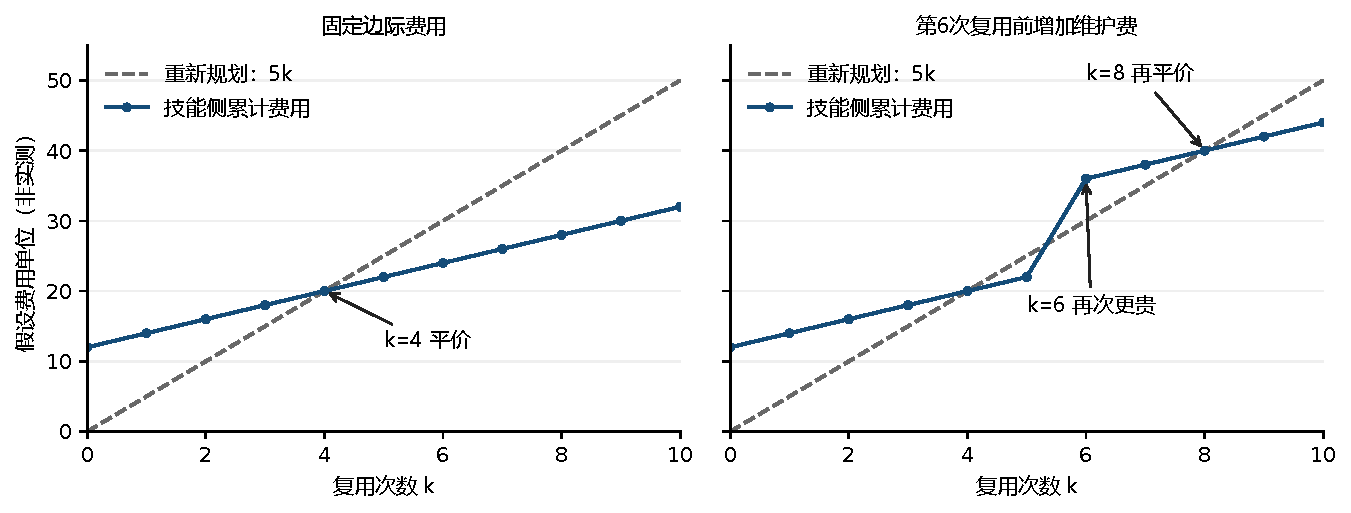
\includegraphics[width=0.98\linewidth]{figures/generated/ch08-cost-teaching.pdf}

\caption{构造的费用模型：左侧固定准备与复用费用在 $k=4$ 平价；右侧第六次前支付一次维护费，费用关系暂时反转，到 $k=8$ 再平价。全部为教学假设，非 E05 实测或拟合，原数组与公式可复算。}
\label{fig:ch08-kstar}
\end{figure}

% 图主体在 ch08-kstar-body.tex，便于单独编译与复用。
\begin{figure}[htbp]
\centering
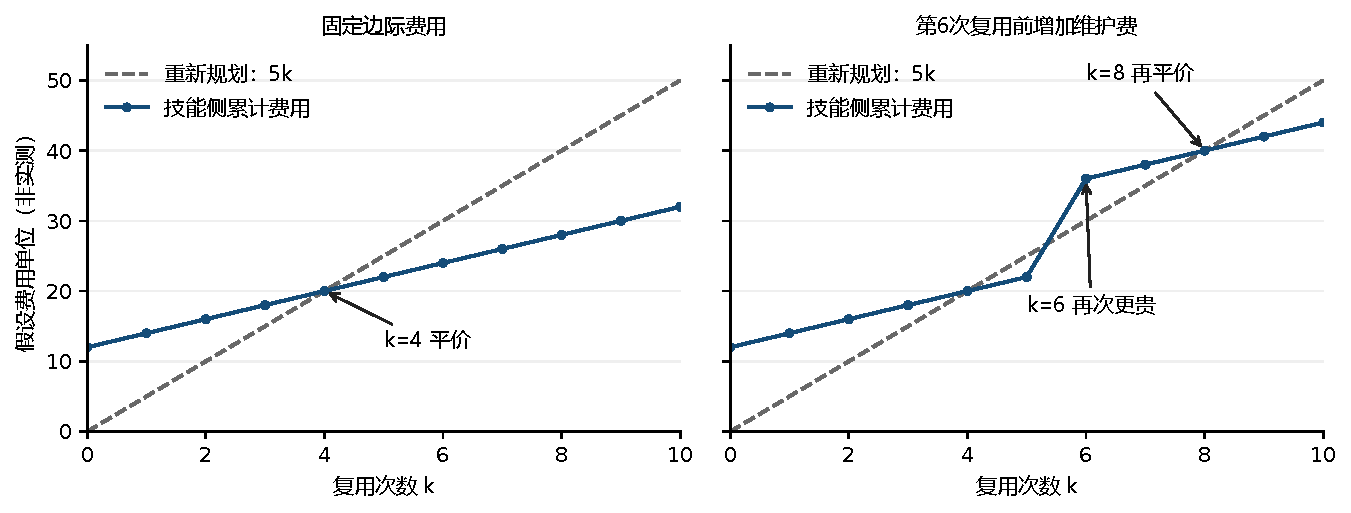
\includegraphics[width=0.98\linewidth]{figures/generated/ch08-cost-teaching.pdf}

\caption{构造的费用模型：左侧固定准备与复用费用在 $k=4$ 平价；右侧第六次前支付一次维护费，费用关系暂时反转，到 $k=8$ 再平价。全部为教学假设，非 E05 实测或拟合，原数组与公式可复算。}
\label{fig:ch08-kstar}
\end{figure}


\subsection{一个能精确复算的教学成本图}

图~\ref{fig:ch08-kstar} 使用明确的\textbf{假设费用单位}。重新规划没有额外准备费用，每次需要五单位；技能准备需要十二单位，每次复用需要两单位。因此两条线为 $5k$ 与 $12+2k$，按式~\ref{eq:ch08-integer-threshold}，最早在\calcnum{$k=4$}时平价，最早在\calcnum{$k=5$}时严格节省。它说明固定成本和边际成本如何共同决定交点，不是对任何真实模型调用价格的拟合。

右图保持同样条件，但假设第六次复用前必须支付十二单位维护费。第五次复用时，技能累计二十二单位，低于重新规划的二十五单位；到第六次，技能累计三十六单位，高于重新规划的三十单位；到第八次又达到四十单位平价。这些都是本书构造条件下的精确计算，原始数组与公式随图保存。

这个例子同时解释了“首次交点”和“以后始终更便宜”的区别。只观察前五次，可能认为技能已经回本；加入后续维护，累计优势却会暂时消失。真实系统的维护时点、费用和失败损失不一定如此规则，因此不能用一条拟合直线替代整个生命周期。若报告一个阈值，应明确它是已观测范围内的首次非正成本差，还是在更强模型假设下推导出的长期阈值。

频率在这里如何进入？如果费用只按调用次数发生，同样十次使用分布在一天或一个月，不改变次数轴上的两条线。若按月需要刷新依赖、资产会过期，或长时间不用后必须重新核验，日历时间才带来额外成本。此时可以写出同时依赖次数和时间的费用，而不能一边沿用纯次数模型，一边声称频率降低必然使次数阈值右移。

\subsection{成功率约束不能从成本线里省掉}

最便宜的策略可能是遇到难题立即停止。若只比较调用费用，它甚至可以击败所有认真实现的技能；对实际任务却没有意义。成本比较应在明确的质量要求下进行，或者并列报告成本与质量，避免把减少有效工作误读成效率。

一种做法是预先规定可以接受的性能损失，再检查技能方案是否满足相应约束；另一种是保留质量与费用两个维度，不把它们合成单一分数。若采用失败惩罚加权总费用，惩罚权重应有任务依据，并做敏感性分析。不能在看到结果后调大某项权重，使偏好的方案刚好成为最优。

E05 v2 的动态组提供了很直接的提醒：来源任务格式失败使其较早停止，调用账可能因此变小，后续又没有有效技能。把这种轨迹压成一个平均费用，会让工程失败看起来像高效策略。完整结果应同时列来源通过、准入、实际读取、首轮成功、额外修复和发布事件，成本线才不会脱离行为过程。

\subsection{平均维护费用可能遮住长尾}

两个技能的平均复用成本相同，失败分布却可能完全不同。一个每次都稍贵，另一个大多数时候很便宜，偶尔需要长时间人工排查或大量模型修复。是否接受后一种模式取决于任务的延迟和恢复要求，不能仅凭均值决定。

实验可以报告费用分布、上分位数或超预算次数，但小样本无法稳定估计很罕见的尾部事件。没有观察到昂贵修复，不等于修复费用为零。对于当前仅少量任务的流程试跑，应直接报告修复路径是否被触发；若没有触发，相关成本和成功率属于未观测，而不是完美表现。

技能退役也有成本。删除一份代码可能很便宜，识别它的所有调用者、迁移依赖、清理旧检索索引和验证替代版本却不一定便宜。生命周期账应允许这些费用出现。若研究只覆盖创建与短期复用，就如实限定范围，不把这一小段累计费用称为长期拥有成本。

\subsection{有缺失费用时，宁可保留区间也不要制造交点}

费用缺失与费用为零是不同状态。一次外部请求超时，应用可能没有收到 usage，但服务端可能已经执行；一次恢复运行只加载任务结果，也可能漏掉之前的构建账。若把这两种情况都填成零，成本较低的一方可能只是记录更不完整。图上的交点越精确，这种误解反而越隐蔽。

若能为缺失费用给出有依据的上下界，可以将总成本写成相应范围，再检查两个方案的范围是否仍然分离。若缺少合理上界，就应明确该格点的完整成本未知，不能通过平均其他任务来伪造一笔已支付费用。估计值可以作为单独的情景分析，必须与记录值分开。

相同问题也出现在时间账里。逐 episode 的耗时相加，不一定等于用户从提交到完成所经历的总时间；并行任务的耗时总和又可能大于墙钟时间。准备环境、构建索引、等待队列和恢复中断，都可能不在模型响应计时内。报告应分别命名累计执行时间与完整流程墙钟，不把现成字段换一个更宽泛的名字。

成本审计应从最小事件向上求和，再与序列、格点和全局汇总核对。同一事件只能计入一次总账，但可以带有多个分析标签，例如属于修复阶段、使用某个模型、服务某个技能。标签用于分组，不应让同一笔费用在总计中重复出现。E05 旧分析将累计复用调用再乘次数，正是没有守住这一层级关系。

记录不完整并不要求丢弃所有数据。已经保存的任务真值、调用次数和错误轨迹仍有价值，只是支持的主张变窄。可以报告部分成本、确定发生的事件和缺失范围，暂缓完整回本判断。这样比覆盖旧记录后补一张完整表更利于后续修复，也更符合本书对历史运行的处理原则。


% ---------- 5. 条件变化 ----------
\section{怎样设计能区分复用与多算力的试验}
\label{sec:ch08-next-design}

技能方案常常同时拥有来源任务、持久代码、额外提示和失败修复，基线却只拿到当前问题。这样的系统比较可以回答“采用整套流程是否值得”，不能单独回答哪一项造成改进。若想归因于代码参考本身，需要为两边对齐起始信息、当前任务预算和其他反馈，或者将额外信息明确作为干预的一部分。

动态技能与静态技能的比较尤其如此。动态臂多一次修复机会，当前任务结果可以因为额外计算改善，后续任务又可能因为新版本改善。E05 新设计将首轮结果和修复结果分开，避免直接改写主结果；但动态修复还可能为未来任务增加有用经验，因此其总预算仍与静态臂不同。描述这一完整策略是合理的，宣称差异只来自“会更新”则需要进一步对照。

可以加入不写持久物、但拥有相同任务内修复预算的对照，帮助区分额外求解与持久更新。也可以让两条策略都完成相同来源构建，再只向其中一条提供代码参考，检查资产可见性的作用。这些设计会改变所回答的问题，不能在一张表里只保留最有利的对照而不说明关系。下一次真实试验需要先冻结设计与预算，再运行。

\subsection{失败修复：当前任务的第二次机会与下次任务的第一份经验}

一个复用任务失败后，可以继续修当前答案，也可以改供下一题使用的持久物。
两个动作发生在同一时刻，却有不同评价对象：前者影响当前任务最终能否完成，后者影响后续任务的起点。
只报最终成功率会把多一次尝试与更好的持久经验混在一起；只报持久写入次数又看不出写入是否经过验证。
实验需要同时保留首次验收、修复验收和版本发布三个事件。

E05 新版把首次验收固定为主结果。
首次失败后，即使修复成功，原来那一格仍然记录失败，另列修复结果和修复成本。
修复通过且满足准入条件时，才用新条目替换旧参考；修复失败则保持原来的有效条目。
如果旧库本来为空，修复失败后仍然为空，不能为了使动态臂``确实发生了更新''而把失败代码硬塞进去。

修订预算必须带着作用范围一起书写。
``每次复用机会允许一次修复''与``整段任务序列允许一次修复''会产生不同的额外调用量。
旧协议采用前一种单位，因此在每次机会重新计数并不自动违反那份文字协议；
本书 v2 主动采用后一种单位，使预算对象成为一个任务族、一个格点、一次重复构成的完整序列。
这是实验设计的改动，不能在旧运行剩余的两块上换上新逻辑，再把全部结果并成同一组。

预算耗尽描述的是\textbf{不再给予修复机会}，不是另一个任务真值。
当前任务仍按实际验收记成功或失败，额外标记``修复被预算拒绝''。
把超预算另立为既非成功也非失败的类别，再从成功率分母中排除，会使失败较多、较早耗尽预算的策略得到不恰当的统计待遇。
完整账本应让读者同时看到：失败多少次、请求修复多少次、准许多少次、修复成功多少次、最终发布多少次。

\subsection{复用格点是否共享同一条前缀}

一种设计从同一份来源技能连续运行后续任务，在第零、第一、第二和第四次复用处读取累计费用。它能直接观察一条生命周期的前缀，但各格点高度相关，后续任务也受前面更新影响。另一种设计为每个格点独立重建技能、独立运行相应长度的序列，格点之间包含来源生成的随机差异。两者都可采用，解释却不同。

E05 新协议采用独立格点：每个任务族、格点和重复构成一条重新建立的序列。因而不同格点的构建费用可能不同，成本曲线不是同一个技能生命周期的连续采样。不能从独立格点的波动直接推出某条技能在第几次发生维护，也不能将较小格点的构建费用替换进较大格点以获得更平滑曲线。

如果目标是估计真实部署的一段连续使用过程，应另外安排共享前缀的任务流，并保留状态演化。若目标是比较不同预期复用长度下的重新部署成本，独立格点更贴近该问题。选择设计时应从使用情景出发，不应因为某种图更好看就混用两者。

\subsection{任务族的重复与独立证据}

同一模板下替换几个常数，确实可以产生不同输入，但不一定提供新的机制覆盖。若所有任务都考察闭区间端点，重复再多也很难说明技能对状态管理或异常契约有效。任务族内重复可以估计当前机制下的随机波动，跨族覆盖则关系到适用范围，两者不能互相替代。

一个小规模试跑更适合回答装置问题：技能是否进入提示、来源失败是否被拒绝、修复预算是否正确扣除、恢复运行是否重复计费。它可以据此发现下一轮值得修复的问题，却不应被迫承担普遍临界次数的证明。把每项运行的用途写清，比让所有运行都输出一个看似完整的命题结论更可靠。

当前v3只有离线验证，沿用的执行路径尚不具备经验证的操作系统隔离；v4仅有受限文件工具草案，没有完整运行器。本版仍缺完整技能依赖图、自动退役和真实接口变更回归数据，也未验证返回语义漂移判据。后续试验需要先完成执行边界与资源记录，再冻结任务独立性、质量约束和比较单位。

\section{条件变化：换环境、换模型、换接口}
\label{sec:ch08-conditions}

\begin{itemize}
  \item \textbf{换环境。}Voyager 在重置的新世界中进行零样本评价（表~\ref{tab:ch08-voyager}）。
        所报迭代数的差距方向一致，证据范围为 \cited{3} 次运行、\cited{4} 个任务。
  \item \textbf{换模型。}原文 GPT-4 版本发现的独特物品数是 GPT-3.5 版本的\cited{5.7}倍（Fig~9），
        而原论文当时报告的 GPT-4 API 价格是 GPT-3.5 的 \cited{15} 倍\cite{voyager-2305}。
        比较带技能库系统的表现与费用时，需要同时报告代码生成模型。
        该对照同时改变技能生成与执行决策，所得差异属于整套系统。固定技能资产的迁移还需要保持资产不变，单独替换读取者。
  \item \textbf{换接口。}高层 API 变化可能造成显式报错或静默的语义失效。
        Voyager 的报告里没有接口版本变更的对照\cite{voyager-2305}；
        2608.03392 把``组件退役''与``回滚成功率与成本''列为应当报告的度量\cite{coding-survey-2608}，
        这是一项评价要求，不能据此概括全部方法都没有相关数值。\textbf{本章尚无接口升级后的真实对照数据。}
  \item \textbf{重复率下降。}复用频率决定需要等待多久，才能累积到某个使用次数。
        在仅按次数计费的固定成本模型中，频率不改变次数轴上的交点；若还存在按时间发生的维护或过期，日历节奏才会进入成本模型。
        若实际使用次数达不到所需阈值，即使技能在每次调用中都有效，也可能无法收回准备费用。
        因此报 $k^{*}$ 时，应同时给出观察时间窗口及实际或预期使用量。
  \item \textbf{技能库增大。}候选池变大而注入条数固定（Voyager 取 \cited{5} 条），
        不能据此预定检索方差必然上升；需要同时观测检索费用、适用候选召回与误调用。相关成本既可能体现为费用，也可能体现为失败。
        因此技能库的规模必须与误用率一起报告，
        单报规模既不能证明收益，也会遗漏检索和维护费用。
  \item \textbf{检索与误调用的代价变化。}        检索要付算力与延迟，误调用一次要付调试与回滚。
        这两笔费用应按实际发生阶段计入，
        若这些费用增加在每次复用上、其他条件固定，就可能提高复用成本，使原交点右移甚至不再出现；一次性费用则改变累计成本的起点，不能都算作斜率。\emph{检索做得更好与技能更划算不是同一件事}——
        检索可能增加计算也可能减少误用，交点变化方向应由两者合计后的实际成本决定。
\end{itemize}

% ---------- 6. 选择原则 ----------
\section{选择原则}
\label{sec:ch08-choice}

\begin{enumerate}
  \item \textbf{把``该不该固化''做成一次带验收的判决，而不是生成的副产品。}
        最小要求是记录：这次固化依据的是哪几次执行，判定者是谁，有没有被反驳过。
  \item \textbf{技能元数据必须含不适用条件。}
        只写适用条件时，库增长可能增加不合适候选；是否提高误用率必须另测，不能预设单调关系。
  \item \textbf{回本点要用成本曲线算，不要用复用次数猜。}
        固化那一次的调用与 token 要计入；$k$ 数的是同一件事的重复次数。
  \item \textbf{被引用者变更时，依赖它的组合技能必须重新验证。}
        版本及依赖记录有助于找出受影响集合，应纳入维护流程。
  \item \textbf{报告技能库收益时，同时报告基础模型与接口版本。}
        少了这两栏，数字无法跨报告比较（见 §\ref{sec:ch08-conditions} 的换模型一项）。
\end{enumerate}

% ---------- 7. 反例 ----------
\begin{pitfallbox}
\textbf{反例一：把``这次跑通了''当成技能成立。}
Voyager 自陈 self-verification 偶尔判错、课程偶尔提出不可达任务、
生成的代码偶尔调用不存在的 API\cite{voyager-2305}。
跑通一次只说明这一次的参数与环境下它能跑，不说明它描述了那件重复发生的事。

\textbf{反例二：把库变大当成能力变大。}
检索固定取 \cited{5} 条\cite{voyager-2305}，库增长后候选集合变化，但仅凭条数不能推出检索方差的方向。
2608.03392 把``组件退役''列为应当报告的度量\cite{coding-survey-2608}，
原论文未给出完整退役对照，本书不据此证明库规模与质量的必然关系。

\textbf{反例三：把换模型后还能跑当成技能可移植。}
GPT-3.5 下发现物品数是 GPT-4 下的 \calcnum{1/5.7}\cite{voyager-2305}。
这是替换代码生成模型后的整套系统对照。评价技能资产的可移植性，还需固定技能版本，并报告两个读取模型各自的无技能库基线。

\textbf{反例四：把复用次数当成回本点。}
回本点是成本线的交点（图~\ref{fig:ch08-kstar}），
Voyager 的成本段没有``回本所需任务数''这一项\cite{voyager-2305}。
用``复用了三次所以值了''来替代成本计算，等于把固定成本那一笔划掉。
\end{pitfallbox}

\section*{习题}
\begin{enumerate}[label=8-\arabic*.,ref=8-\arabic*]
  \item\label{ex:ch08-1} 选一个你正在用的技能库，统计其中有多少条元数据里有``不适用条件''这一项。
        如果没有，估算误用率随库规模的变化需要额外记录什么。
  \item\label{ex:ch08-2} 表~\ref{tab:ch08-voyager} 在相同的最大提示迭代预算下比较有无技能库。
        它已经提供什么证据？若进一步比较包含来源构建费用的总资源效率，还缺哪些记录与对照？
  \item\label{ex:ch08-3} 先用式~\ref{eq:ch08-integer-threshold} 区分平价与严格节省的最早次数，再检查图~\ref{fig:ch08-kstar} 右侧加入的维护费用。
        若维护费用更高或更早发生，请计算哪些格点的成本关系会改变。
  \item\label{ex:ch08-4} 本章说``本章尚无接口升级后的真实对照数据''。
        请设计一个最小实验，使得``接口变化后有多少已入库技能静默失效''这个数可以被测出来。
\end{enumerate}

\section*{常见误解}
\begin{itemize}
  \item \textbf{``代码技能比文本记忆更可靠，因为能跑''。}
        能跑只验收了这一次执行。Voyager 自陈生成的代码偶尔调用不存在的 API\cite{voyager-2305}——
        部分这类错误在执行前可由接口检查发现，不能只依赖最终运行。
  \item \textbf{``技能越多越好''。}
        检索只取 \cited{5} 条\cite{voyager-2305}，多出来的部分不进入上下文，
        它们仍可能影响检索与维护，方向和大小需要测量，不能自动当作成本增加。
  \item \textbf{``消融掉了技能库还更差，说明技能库有用''。}
        在其他条件受控时，这可以提供技能库贡献的证据；但它不足以回答P4：P4 说的是存在临界重复次数，
        需要的是成本曲线，消融给的是有/无的二分对照。
  \item \textbf{``技能库跨任务复用，所以它是通用的''。}
        原文换代码生成模型后发现物品数相差 \cited{5.7} 倍，这不是冻结同一技能库后换读取者的实验\cite{voyager-2305}。
        可复用与可移植是两件事，第 5 章的 E03c 检验的是后者，当前 P3b 仍未判定。
\end{itemize}

\section*{进一步阅读}
\begin{itemize}
  \item \cite{voyager-2305}：本章 Voyager 相关数字的出处，E05数字另有本书原始记录。
        Sec~2.2 与 Fig~4 是技能库结构；Table~2 是表~\ref{tab:ch08-voyager}；
        Sec~3.4 的消融（随机课程 \cited{-93\%}、去 self-verification \cited{-73\%}）与
        Sec~4 的成本段（GPT-4 比 GPT-3.5 贵 \cited{15} 倍）是本章反例一与反例四的来源。
        读它时注意：``回本所需任务数''是未定位项。
  \item \cite{coding-survey-2608}：六类持久演化目标里 skill and tool 的位置（§3，Table~3），
        以及 §5.2 那份把``组件退役''与``回滚成本''列为度量的清单。
        本书使用v3的章节定位；引用时不要把``应当报告''读成``已经报告''。
  \item \cite{ksi-2607}：\texttt{applies\_when} / \texttt{does\_not\_apply\_when} 的出处，
        本章 §\ref{sec:ch08-interface} 把它搬到了技能元数据上。
  \item 本书第 4 章：验证层级四级与六类代码信号的分布，
        \cited{75.4\%} 依赖可执行验证那个数字解释了本章的域边界。
  \item 本书第 5 章：两种拟合目标与 E03c。技能是最容易被写成``拟合到求解器''的一种持久物，
        因为它的正确性常常依赖那个模型会不会写出正确的调用。
\end{itemize}
